\chapter{Literature Review}

\label{ch:background} 

\section {Background study and Traditional applications}
The traditional systems currently in the market are providing various news data like popular ones and breaking news for its readers. The increasing number of mobile phones contribute to large number of news readers in mobile phones and tablets. To maintain this growing population towards news-reading and to meet their expectations there is an excessive need of adaptive personalization to suit individual taste and interests which is limited in traditional systems.\newline
Several applications in the marketplace were reviewed before giving a kick start for the project. For Example, \textbf{BBC News app} personalization works in a way letting the user to customize the ares of interests and populate '\textbf{My News}' page accordingly. It works more towards user-customization but lacks adaptability and presents outdated content if there aren't any recent news which makes it bit awful \cite{gitsham_2015}.\newline
Others work in a way aggregating news from various sources which are knows as 'News Aggregators'. One such example is \textbf{Flipboard} which works in a way allowing users to pick their favorite stories from various sources or categories and populate most relevant content. Additionally it has Machine learning algorithms which learns from users interactions like follow, flip and heart and populate contents based on the high interactions\cite{anne_2018}. \newline

And there is an observation made on \textbf{Google News} personalization which works considering two approaches. 
\begin{itemize}
    \item Taking users past click logs 
    \item Building user profiles from personal preferences and interests \cite{googlenews}.
\end{itemize}
Also, according to recent research, about \textbf{60 percent} of the applications follow hybrid recommendation system \cite{recommend_2020}.The hybrid recommendation system refers to the efficient combination of content based filtering and collaborative filtering approaches.This enhances the accuracy of the recommendations quite well\cite{Jonnalagedda_2016}.\newline

\textbf{Experimental Investigation}\newline
And in my research and analysis I came across one brief experimental analysis on my current work which gave me more clear picture what is the exact problem situation and why its more important. According to the experimental investigation, while a gigantic and enormous amount of news gets released every hour, it creates a challenging situation to gather all the news from the right source and recommend the right news to the users that too match their reading preference as much as possible.\cite{Li2011}. This issue is termed Personalized News Recommendation by the authors. This paper also insisted we get huge resources of news information across the world through the internet and the recommendation system has to wisely recommend the news for the user's based on user profile and news content to the readers which is why this issue is more important to consider. This research study has provided detailed understanding of existing personal news recommendation systems and helped to identify the importance and enhancements to pick from there. 
The research work explains the different methods of recommenders which are Content-based Methods, Collaborative filtering and the hybrid recommendations which helped in understanding different approaches and choose the right-most one.
\newline
\textbf{User Profiling}\newline
Another major challenge is to construct the user profile. The user profiling is important to provide the preferred news articles to the readers from a wide range of sources. One of the research papers which explains briefly on User Profiling for News personalization. This paper follows an approach for user profile building by following the entities the user included in the comments\cite{meguebli2014building}. These entities are then extracted from each news article for constructing the user profile and recommending similar articles which the user has commented. This helped in getting more clear on the concepts of user profile and what are different ways to build them for each user. 
This gives an understanding of using comments which are some sort of user interactions and recommend news articles based on that. \newline

\textbf{Location Preference}\newline
There is a research study which states that adding location preference to the news recommendation system helps in increasing the customer satisfaction from 8.6 to 9.4. The combination of user profiling, popularity and location improves the customer satisfaction and enhances the application to a desired level\cite{Natarajan2016}.\newline

\textbf{Theoretical Architecture of News Recommendation System}\newline
 A research paper proposes the overview of the structure of recommendation system and the overall functioning elements.\newline
 There are three major components in the system which are the user component, correlation table and the ranking filter. \newline
 \begin{itemize}
     \item \textbf{User Component: }

 The user component comprises the user attributes characteristics, user behaviour characteristics. User Attribute characteristics as stated in the paper indicates the user demographic elements.User behavior characteristics are of two types as stated by the author which are implicit and explicit types. The explicit types are the ones which are tracked from direct user interactions and the implicit types are derived from the browser history and so on\cite{Li2019}.  
 
  \item \textbf{ Correlation Table: }
  The user information along with the collaborative filtering outputs like Item-Item, User-Item,  User-User correlation information forms the correlation table and provides the input for the recommendation filter.
  
  \item{Ranking algorithm: }
  The final step is to provide the filtered set of recommendation results going through optimization removing all the blacklists and providing the refined list of news articles for the readers. This is processed through some specific ranking algorithm and finally gives the desired results.
 
  \end{itemize}
  
   \begin{center}
  \begin{figure}[h!]
   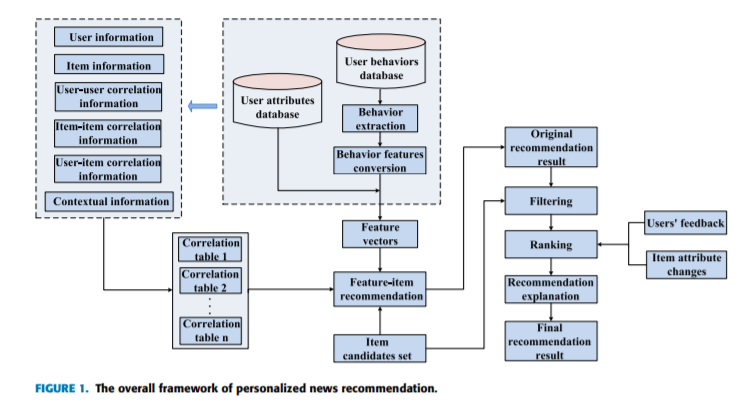
\includegraphics[scale=0.7,width=7in,height=4.5in]{images/systemdesign.PNG}
    \caption{System Architecture}
    \end{figure}
    \end{center}
    
\textbf{Recommendation Model}\newline
The overall system design is supposed to work in a workflow model basis which is described as below. Through effective analysis of user information with context details both explicit and implicit, user profile model is created and with the approaches of several types of collaboration filtering or the hybrid approach correlation model is created.Based on the combination of both, user prediction model is developed which recommends the right set of news articles to the readers following the optimized ranking algorithm along with the process. 

The overall process flow model is represented as below. 
 \begin{center}
  \begin{figure}[h!]
   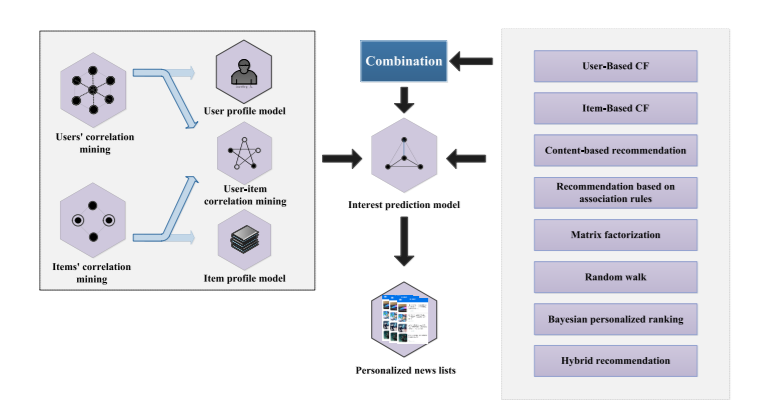
\includegraphics[scale=0.7,width=7in,height=4.5in]{images/ProcessFlow.PNG}
    \caption{System Model}
    \end{figure}
    \end{center}

The literature review was done on various angles and collected information to include as many enhancements and features for the proposed system.
\textbf{Missing features on existing applications}

The applications in the marketplace shows some lag in few features which are considered in our proposed system.
\begin{enumerate}


{ \bf  \large \item Lack of Visual Evidence of Users Interests}\newline
While such applications already exists in the market which learns from users context details like interested categories and interactions, there is a no explicit and user-friendly visualization of what the users favorite zone and order of interests and \textbf{numeric comparisons} of user interests. There is no clear picture of what the users interests are after a many interactions and the system starts to overload the content making it difficult for users to understand what their major interests are over a period of time.

 
{\bf \large \item   Overloaded feeds}\newline
The recommendations and the personal stories are overloaded in the apps sometimes making it a noise. This in-turn affects personalization and leads to criticism if the algorithm is not considering best relationship factors between the users or the relevancy score.

 {\bf \large \item   Minimal or No Scope on Visualization}\newline
The present news app provides more data with but less ideal for users who look for more friendly and appealing visual tools.
\end{enumerate}

\section {Proposed System}
The proposed system works in a way fulfilling three major targets of the application. 

\begin{enumerate}
    \item Personalization
    \item Visualization
    \item Recommendation
\end{enumerate}

This all-in-one system helps enhancing the news app one step further making it more user-friendly and easy to use.

\begin{enumerate}

    {\bf \large \item   Personalization }
    \begin{center}
  \begin{figure}[h!]
   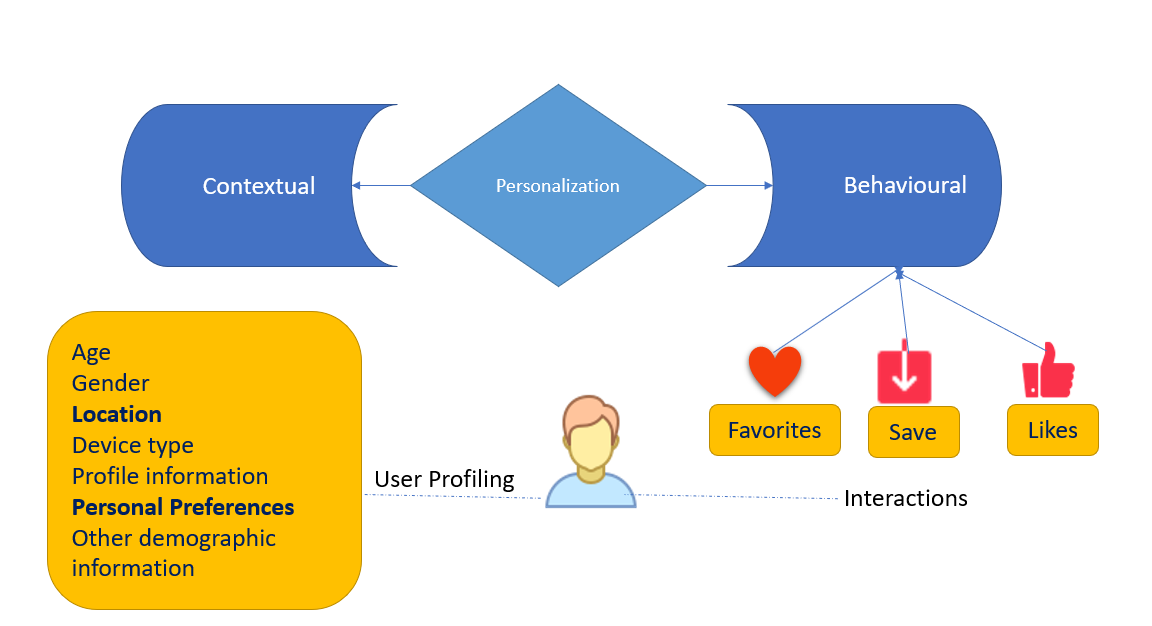
\includegraphics[scale=0.7,width=7in,height=4.5in]{images/personalization.png}
    \caption{Personalization}
    \end{figure}
    \end{center}
    
    Personalization is implemented in this Buzzfeed  application with two possible approaches as shown in the figure.
    \begin{enumerate}
    {\bf  \item \large Contextual Personalization} \newline
  \hspace*{1cm} Contextual personalization is the most widely adopted model where the user profiling is considered for customization and recommendation.
  The user profile is gathered and analysed thoroughly thus understanding individual selected preferences and several other factors expressed during the signup process for creating his/her profile.
  
  It generally comprises several factors including:
  \begin{itemize}
  \item Age
  \item \textbf{Location}
  \item\textbf{ Selected Preferences}
  \item Gender information
  \item Demographic information \cite{authentic.}.
  Personal Buzzfeed considered two of the above Location and Selected Preferences and works with the personal feed.
\end{itemize}
 {\bf \large  \item  Behavioral Personalization} \newline
  \hspace*{1cm}
  Behavioral Personalization is measuring user's every interaction and moves in the application to predict their interests and personalize their feed with most likely items. 
  This is considered more important as it determines the users trending mindset and gets updated with their moods to adapt to their current preferences.
  This is assessed in our application considering three major interactions for loading their personal feed.
  \begin{itemize}
      \item \textbf{Likes} with a thumbs-up icon
      \item \textbf{Favorites} with a heart icon
       \item \textbf{Save} with a download icon
  \end{itemize}
  \end{enumerate}
\textbf{  \large How It All Works}  \newline
   \textbf{ Weight-Map Algorithm } \newline
   For Personalization, the application works out an algorithm called '\textbf{Weight-Map}' Algorithm which takes all combination of Selected preferences from Contextual and other interaction based preferences and sorts the personal feed to present the users with top likes news articles.\newline
    
    
     \textbf{ User Location } \newline
     User location is considered separately and loaded initially with the Global data component and list down the news of his/her location with option to switch to other countries and any categories.
    
    {\bf \large \item   Visualization }\newline
    Visualization is implemented using amcharts which is a library that was integrated into the frontend for accomplishing geographical maps and pie charts.
    
    \textbf{Why Amcharts?}\newline
    Amcharts is chosen for integration as it has good projection of advanced charts and also supports plugins for maps with well-defined projections and compatible with the existing front-end technologies design and development \cite{amcharts_2018}.
    
    \textbf{Where in Buzzfeed?} \newline
    This is implemented in two primary areas in our application.
    
\begin{itemize}
    {\bf \item Map View}
    The amcharts projects globe with all country geodata and initially it loads the user's location data on getting to this component in the frontend with possible option to see any kind of category the user likes to know in this location.
    The globe is clickable and allows to switch to any country and loads respective news based on selected category.
    
   { \bf \item User charts }
   The amcharts makes it possible to project any kind of data having advanced chart types. Each user interests are mapped with respective preference weights associated for various category items in the news feed an they are represented in terms of pie-chrts to let users know explicitly what their interests and zones are. 
   
\end{itemize}

    {\bf \large \item   Recommendation }\newline
    Recommendation is another area where the users interests are analysed and compared with other similar users and suggested some categories which they might be interested in. They are a kind of Machine learning algorithms which learns the users and provide relevant and optimal recommendations \cite{mishra}. This is accomplished using \textbf{Apache Mahout Recommendation System}.
    
    There are many types of recommendations possible like popularity-based recommendations, Content-based recommendations, Collaborative recommendation systems,etc 
    \begin{center}
    \begin{figure}[h!]
    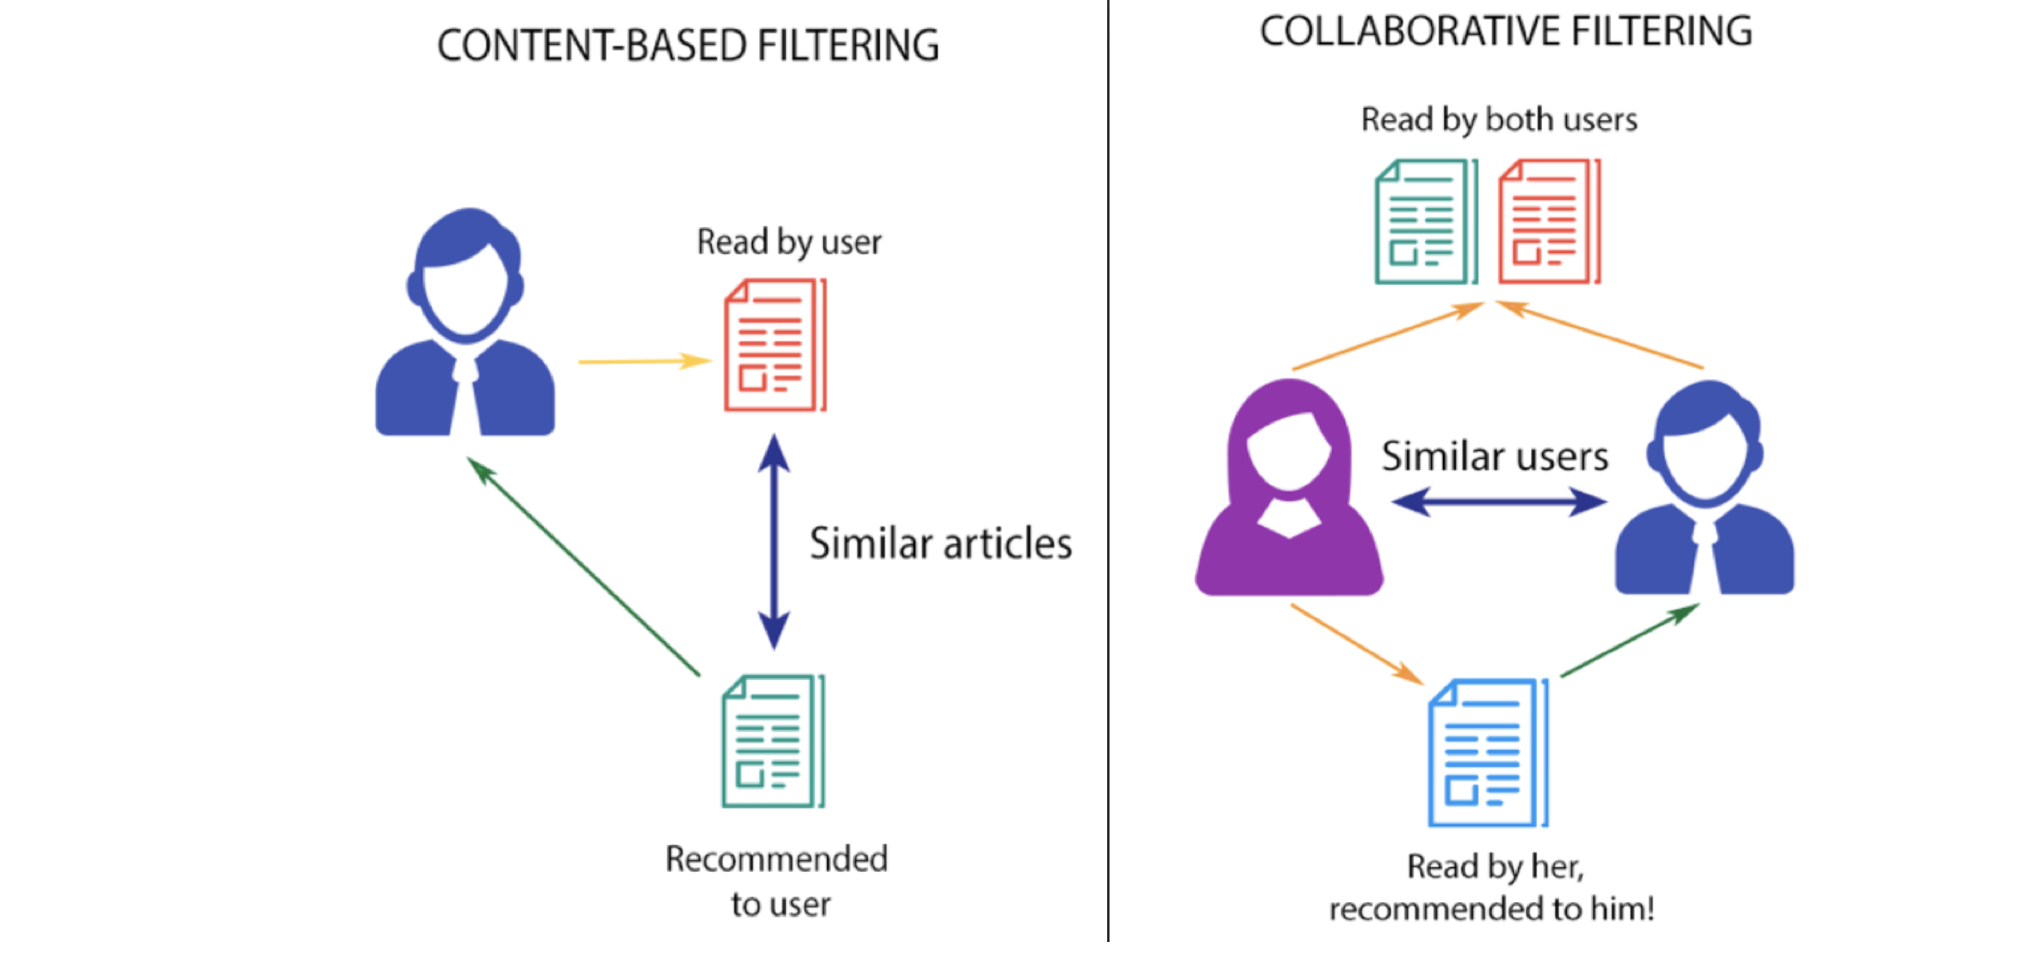
\includegraphics[scale=0.7,width=7in,height=4.5in]{images/recommendation system.png}
    \centering \caption{Recommendation Types}
    \end{figure}
        \end{center}
   \begin{enumerate}
      \item\textbf{ Content-based Recommendations:}
            Content-based Recommender system recommends the things or similar items which are most liked by the user.
            It observes the users like patterns and search history and recommends similar items to the users.
   \item\textbf{ Collaborative Filtering:} 
            Collaborative filtering is the highly beneficial and effective methods of recommendation system being implemented and provided high success rates in many companies. For example, Amazon recommendation system which suggests on selecting a product, a pair of other products being bought together or similar products bought by other users which has increased sales by 29\%. Other similar success use cases with Collaborative filtering are Netflix movie rentals by 60\% and Google news click-through rates increased by 30.9\% \cite{lee2015a}.
   \end{enumerate}
\textbf{ Reason for Opting Collaborative Filtering} \newline
  So, similar seeing increase in success rates on recommendations with collaborative filtering, this application too incorporates the Collaborative recommendation system comparing similar interests of users and recommend news articles.
  
\textbf{ Why Apache Mahout?} \newline
    Apache Mahout is a popular Apache-licensed open-source library for scalable machine learning algorithms \cite{mahout_2012}. 
    Mahout provides most useful frameworks for Collaborative Filtering implementation. It has in-built framework, functionalities and APIs for machine learning algorithms to achieve the appropriate recommendations to users.
    
\end{enumerate}
    


